Given the size of the data our software will be working on, it requires an efficient way of storing them. There are 2 kinds of data, on the first hand the ones the programs works on; on the other hand, the parameters and utilities.
\subsection{Representation of the playouts}
\subsubsection{Bitboards}
Boards are stored as bitboard. As the game is played on a \ensuremath{8\times8} board, it is convenient to use a 64 bit integer to store the position of the pieces. That way, each and every kind of pieces are stored on the same x64 integer, saving space as opposed to a matrix \ensuremath{8\times8} retaining all the informations. Players own rabbits, cats, dogs, horses, camel and elephant; thus using 6 integers for each player do the job. Adding an additionnal bitboard to store the position of every pieces of each players helps to increase the speed of the algorithm by reducing the number of test required to be done during the playout phases. It also allows quick tests and modifications such as bit twiddling given the nature of the data.

\subsubsection{Nodes}
\begin{figure}[H] 
\centerline{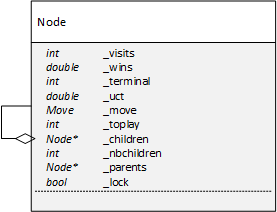
\includegraphics[scale=0.8]{Data_Structure/Img/Node.png}}
\caption{\label{fig:nodedetails}\textit{Details of the data cointained in a node}.}
\end{figure}
Nodes contain statistics about the previous results, a pointer to their parent, a pointer to the first of their children and the number of children they own. They are stored in an array (\textit{\_tree}) set at the begining of the program, thus grouping them on a countinuous memory segment. Therefore the time to gain access to them is decreased.

\subsubsection{Prunning}
\begin{figure}[H] 
\centerline{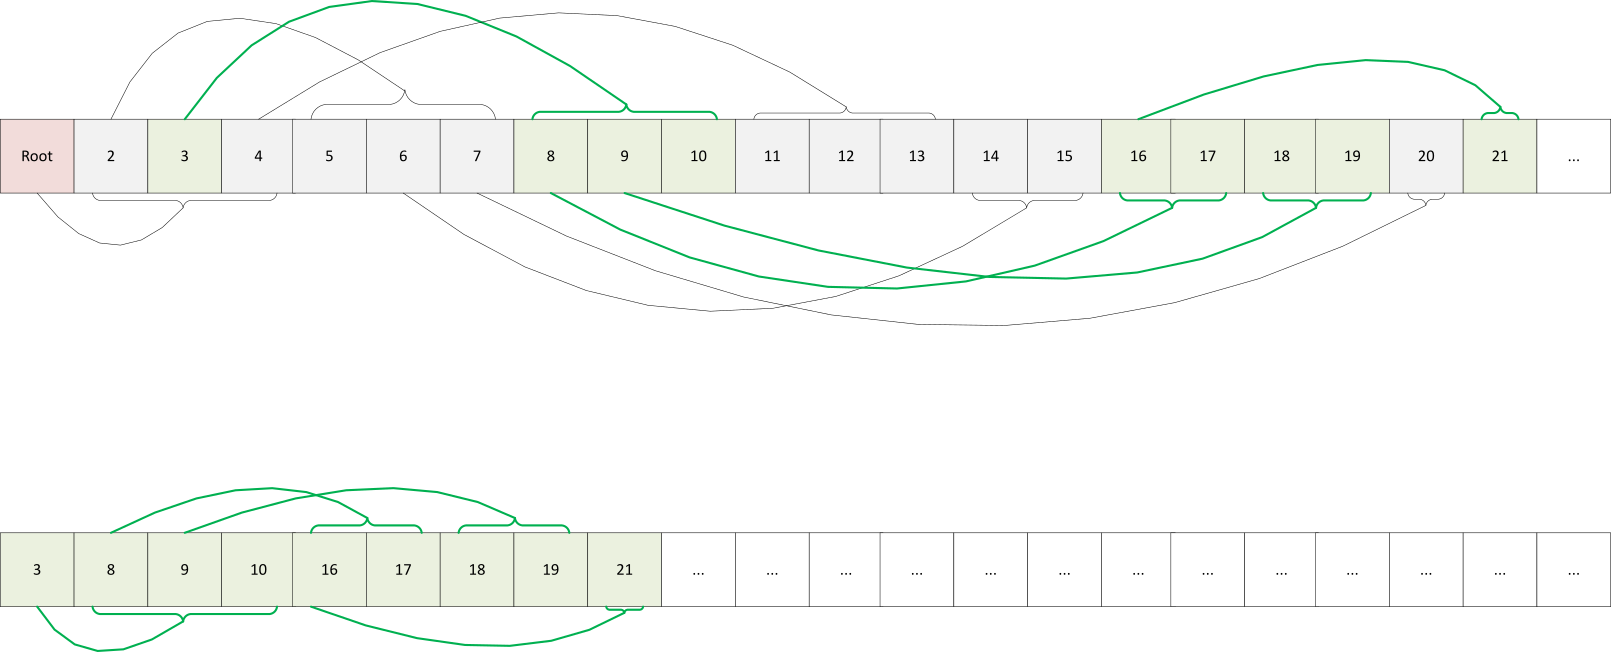
\includegraphics[width=\textwidth]{Data_Structure/Img/array.png}}
\caption{\label{fig:arrayprunning}\textit{Prunning of the tree (before and after)}.}
\end{figure}
In order to prune the tree, we use the following method : create a copy of the current tree (\textit{\_tree}) into a buffer (\textit{\_buff}). The root of the buffer tree will be a copy the chosen node. Then the children are saved going down through the branches. The advantage of this method is that you only copy the nodes you want to keep. However the memory used by the buffer needs to be the same as the one of the tree before the prunning. Thus the maximum memory that can be used by the tree (\textit{\_tree}) is half the memory used by the program. In order to dermine the number of leaves to be created, the program checks how much memory there is left on the computer and use a fixed percentage of it.
\begin{equation}
N = \frac{R \times 90\%}{2}
\end{equation}
\ensuremath{N} = number of leaves.\\
\ensuremath{R} = RAM left to use.

We chose to limit the memory used by the tree to 90\% of the available memory in order to not overload the RAM and to let some left for other operations such as simulations. It also allows us to make sure that the swap will not be used to store the tree as it impacts heavily on the speed of its exploration.

\subsubsection{Game abstraction}
\begin{figure}[H] 
\centerline{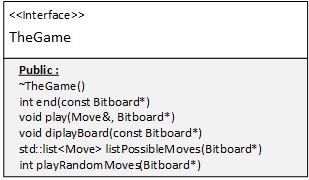
\includegraphics[scale=0.8]{Data_Structure/Img/TheGame.png}}
\caption{\label{fig:thegamedetails}\textit{Details of methods cointained in the interface TheGame}.}
\end{figure}
In order to know the moves that can be played and the winning conditions, the mcts algorithm has to have access to a class describing the game. This abstract class is implemented and passed as a parameter at the instantiation of the mcts object. It allows genericity in the algorithm and permits to use it on any board games such as Connect4 or Arimaa. This interface has 4 main methods : 

\noindent
\textit{\textbf{end}} : check if the board provided is a final state.
\medskip\\
\textit{\textbf{play}} : play a given move on a given board.
\medskip\\
\textit{\textbf{listPossibleMoves}} : list all the possible moves given a board, this is used when a node is to be expanded.
\medskip\\
\textit{\textbf{playRandomMoves}} : play random moves until a final state is reached and return the winner, this is the random simulation part.

\newpage
\subsection{Parameters and utilities}
\subsubsection{Parameters}
Instead of directly passing all the parameters to the mcts object at its instantiation, we decided to create an object that would provide them, given appropriate inline getters. The point of this is to allow quick modification on the parameters without having to rewrite some parts of the mcts to make sure that each files is updated. The main idea applied here is to separate the data from the algorithm with the same principle as the MVC design pattern.
\begin{figure}[H] 
\centerline{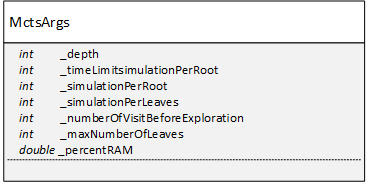
\includegraphics[scale=0.8]{Data_Structure/Img/MctsArgs.png}}
\caption{\label{fig:mctsargsuml}\textit{Details of the parameters of the algorithm}.}
\end{figure}

\subsubsection{Fast log}
The MCTS algorithm does not require an exact value of the \ensuremath{ln(x)} function in order to calculate the UCT value of a node. As numbers are stored in binary on computers, it is more interesting to get  their log in base 2 and to divide it by \ensuremath{ln(2)}. 
\begin{equation}
ln(x) = \frac{log2(x)}{ln(2)}
\end{equation}
\begin{equation}
ln(x) = log2(x) \times \frac{1}{ln(2)}
\end{equation}
\begin{equation}
ln(x) = log2(x) \times 0.69314718f
\end{equation}
Depending on the main operating system (Windows or Linux), the calculus of \ensuremath{log2(x)} will differ. On linux, a quadratic approximation is made, for more details, refer to annexes\ref{subsec:fastLog}. On windows, \textit{\_BitScanReverse64(\&y, x)} is slightly faster. 

\subsubsection{Random numbers : Mersenne Twister}
Given the number of playouts to be simulated, the MCTS algorithm requires a fast random number generator. The Mersenne Twister which is implemented in the STL is faster than the basic rand() function. Therefore we decided to use it.


